% AER E 361 Mission Report Template
% Spring 2023
% Template created by Yiqi Liang and Professor Matthew Nelson

% Document Configuration DO NOT CHANGE
\documentclass[12 pt]{report}
% --------------------LaTeX Packages---------------------------------
% The following are packages that are used in this report.
% DO NOT CHANGE ANY OF THE FOLLOWING OR YOUR REPORT WILL NOT COMPILE
% -------------------------------------------------------------------

\usepackage{hyperref}
\usepackage{parskip}
\usepackage{titlesec}
\usepackage{titling}
\usepackage{graphicx}
\usepackage{graphviz}
\usepackage[T1]{fontenc}
\usepackage{titlesec, blindtext, color} %for LessIsMore style
\usepackage{tcolorbox} %for references box
\usepackage[hmargin=1in,vmargin=1in]{geometry} % use 1 inch margins
\usepackage{float}
\usepackage{tikz}
\usepackage{svg} % Allows for SVG Vector graphics
\usepackage{textcomp, gensymb} %for degree symbol
\hypersetup{
	colorlinks=true,
	linkcolor=blue,
	urlcolor=cyan,
}
\usepackage{biblatex}
\addbibresource{lab-report-bib.bib}
\usepackage{amsmath}
\usepackage{listings}
\usepackage{multicol}
\usepackage{array}

\usepackage{hologo} %KYR: for \BibTeX
%\usepackage{algpseudocode}
%\usepackage{algorithm}
% This configures items for code listings in the document
\usepackage{xcolor}

\usepackage{fancyhdr} % Headers/Footers
\usepackage{siunitx} % SI units

\definecolor{commentsColor}{rgb}{0.497495, 0.497587, 0.497464}
\definecolor{keywordsColor}{rgb}{0.000000, 0.000000, 0.635294}
\definecolor{stringColor}{rgb}{0.558215, 0.000000, 0.135316}
\definecolor{mygreen}{rgb}{0,0.6,0}
\definecolor{mygray}{rgb}{0.5,0.5,0.5}
\definecolor{mymauve}{rgb}{0.58,0,0.82}

\lstdefinestyle{customc}{
  belowcaptionskip=1\baselineskip,
  breaklines=true,
  frame=L,
  xleftmargin=\parindent,
  language=C,
  showstringspaces=false,
  basicstyle=\footnotesize\ttfamily,
  keywordstyle=\bfseries\color{green!40!black},
  commentstyle=\itshape\color{purple!40!black},
  identifierstyle=\color{blue},
  stringstyle=\color{orange},
 }

 \lstset{ %
  backgroundcolor=\color{white},   % choose the background color; you must add \usepackage{color} or \usepackage{xcolor}
  basicstyle=\footnotesize,        % the size of the fonts that are used for the code
  breakatwhitespace=false,         % sets if automatic breaks should only happen at whitespace
  breaklines=true,                 % sets automatic line breaking
  captionpos=b,                    % sets the caption-position to bottom
  commentstyle=\color{commentsColor}\textit,    % comment style
  deletekeywords={...},            % if you want to delete keywords from the given language
  escapeinside={\%*}{*)},          % if you want to add LaTeX within your code
  extendedchars=true,              % lets you use non-ASCII characters; for 8-bits encodings only, does not work with UTF-8
  frame=tb,	                   	   % adds a frame around the code
  keepspaces=true,                 % keeps spaces in text, useful for keeping indentation of code (possibly needs columns=flexible)
  keywordstyle=\color{keywordsColor}\bfseries,       % keyword style
  language=Python,                 % the language of the code (can be overrided per snippet)
  otherkeywords={*,...},           % if you want to add more keywords to the set
  numbers=left,                    % where to put the line-numbers; possible values are (none, left, right)
  numbersep=8pt,                   % how far the line-numbers are from the code
  numberstyle=\tiny\color{commentsColor}, % the style that is used for the line-numbers
  rulecolor=\color{black},         % if not set, the frame-color may be changed on line-breaks within not-black text (e.g. comments (green here))
  showspaces=false,                % show spaces everywhere adding particular underscores; it overrides 'showstringspaces'
  showstringspaces=false,          % underline spaces within strings only
  showtabs=false,                  % show tabs within strings adding particular underscores
  stepnumber=1,                    % the step between two line-numbers. If it's 1, each line will be numbered
  stringstyle=\color{stringColor}, % string literal style
  tabsize=2,	                   % sets default tabsize to 2 spaces
  title=\lstname,                  % show the filename of files included with \lstinputlisting; also try caption instead of title
  columns=fixed                    % Using fixed column width (for e.g. nice alignment)
}

\lstdefinestyle{customasm}{
  belowcaptionskip=1\baselineskip,
  frame=L,
  xleftmargin=\parindent,
  language=[x86masm]Assembler,
  basicstyle=\footnotesize\ttfamily,
  commentstyle=\itshape\color{purple!40!black},
}

\lstset{escapechar=@,style=customc}


\titlelabel{\thetitle.\quad}

% From here on out you can start editing your document
\newcommand{\subtitle}[1]{%
  \posttitle{%
    \par\end{center}
    \begin{center}\LARGE#1\end{center}
    \vskip0.5em}%
}

\title{\textbf{Iowa State University
\\{\Large Aerospace Engineering}}}
\subtitle{AER E 322 Lab 01\\
		  Practice Experiment and Data Analysis}
\author{Matthew Mehrtens, Peter Mikolitis, and Natsuki Oda}

% Define the headers and footers
\setlength{\headheight}{70.63135pt}
\geometry{head=70.63135pt, includehead=true, includefoot=true}
\fancypagestyle{plain}{
	\fancyhead{}\fancyfoot{} % clears the headers/footers
	\fancyhead[L]{\textbf{AER E 322}}
	\fancyhead[C]{\textbf{Aerospace Structures Laboratory Report}\\
					 \textbf{Lab 01 Practice Experiment and Data Analysis}\\
					 Section 4 Group 2\\
					 Matthew Mehrtens, Peter Mikolitis, and Natsuki Oda\\
					 \today}
	\fancyhead[R]{\textbf{Spring 2023}}
	\fancyfoot[C]{\thepage}
}
\pagestyle{fancy}
\fancyhead{}\fancyfoot{} % clears the headers/footers
\fancyhead[L]{\textbf{AER E 322}}
\fancyhead[C]{\textbf{Aerospace Structures Laboratory Report}\\
			  \textbf{Lab 01 Practice Experiment and Data Analysis}\\
			  Section 4 Group 2\\
			  Matthew Mehrtens, Peter Mikolitis, and Natsuki Oda\\
			  \today}
\fancyhead[R]{\textbf{Spring 2023}}
\fancyfoot[C]{\thepage}

\begin{document}
\maketitle
\tableofcontents

\chapter{Pre-Lab} \label{pre-lab}
\section{Introduction} \label{introduction}
Aircraft wings undergo oscillations and other random forces while in flight. This lab replicates and analyzes some of the forces and oscillations a wing will experience in flight while also serving as an introduction to the PASCO tool kits and data processing. To simulate the wing, we used a cantilevered aluminum beam, and to generate and measure the oscillations, we used a PASCO tool kit---specifically the PASCO wave driver, displacement sensor and motion sensor. There were three rounds of testing; each additional round of testing introduced a new variable into the beam movement that changed the shape of the data. The data was collected using the PASCO tool kit and software provided. After the lab, we analyzed and processed the data in Python to how each variable effected the oscillation of the beam.

\section{Objectives} \label{objectives}
During this lab, our primary objectives were to:
\begin{enumerate}
	\item Learn how to record data under dynamic conditions and analyze or post-process the data.
	\item Observe approximately how a common aerospace structural material might respond to oscillatory forces.
	\item Gain familiarity with the PASCO tool kit and the PASCO Capstone software.
\end{enumerate}

\section{Hypothesis} \label{hypothesis}
\subsection{Test 1} \label{hypothesis-test_1}
We predict this test will provide the cleanest data of the three tests. Since the only force acting on the beam should be from the wave driver, we expect the displacement graph to shown a uniform and steady wave---matching the oscillations of the wave driver. The data from this test should closely match the oscillations of an airplane wing in very steady flight.

\subsection{Test 2} \label{hypothesis-test_2}
This test adds a spring with a hanging weight to the cantilevered beam. Due to the oscillations of the spring-weight system, we expect to see sudden highs and lows in the data corresponding with when the spring is in compression or tension respectively. The data from this test should demonstrate the oscillations of the wing in steady flight if there is an additional oscillatory or vibrational force simultaneously acting on the wing.

\subsection{Test 3} \label{hypothesis-test_3}
This test is similar to Test 2 (see Section \ref{hypothesis-test_2}) except a third significant force has been introduced. Due to the addition of arbitrary impulses being applied by hand to the free end of the beam, we expect the data to show large peaks and dips in the data correlated with the timing of the impulses. The data from this test should demonstrate the oscillations of real flight as described in Section \ref{hypothesis-test_2} but also how the wing might react during periods of high turbulence where sudden, large impulses may act on the wing.

\chapter{Lab Work} \label{lab_work}
\section{Variables} \label{variables}
\subsection{Independent Variables} \label{variables-independent_variables}
\subsubsection{Wave Driver Frequency} \label{variables-independent_variables-wave_drive_frequency}
The frequency of the wave generated by the PASCO wave driver.

\subsubsection{Wave Driver Amplitude} \label{variables-independent_variables-wave_driver_amplitude}
The maximum voltage the wave driver will use when oscillating, proportional to the displacement of the wave driver arm.

\subsubsection{Sampling Frequency} \label{variables-independent_variables-sampling_frequency}
The time intervals at which the PASCO motion sensor or displacement sensor poll the position or displacement of the beam. Sensor with a higher sampling frequency will collect more data in the same amount of time.

\subsubsection{Smoothing Span} \label{variables-independent_variables-smoothing_span}
The number of elements after a given element used to calculate a rolling mean while data processing. A small smoothing span will better preserve the shape of the data; whereas, a larger smoothing span will better reduce noise and outliers.

\subsubsection{Time} \label{variables-independent_variables-time}
Each test was run for exactly \qty{15}{s}, measured in \qty{0.01}{s} intervals.

\subsection{Dependent Variables} \label{variables-dependent_variables}
\subsubsection{Displacement/Position} \label{variables-dependent_variables-displacement-position}
The change in location of the cantilevered beam from its equilibrium position, measured closer to the free end along a perpendicular vertical axis.

\subsubsection{Best Fit Curve} \label{variables-dependent_variablesbest_fit_curve}
The line of best fit or fit curve is a normalized curve matching the raw or smoothed data and depends on the shape and magnitude of the displacement data.

\section{Work Assignments} \label{work_assignments}
Refer to Table \ref{table:work_assignments} for the distribution of work during this lab.
\begin{table}[ht]
\caption{Work assignments for lab 01.}
\begin{center}
	\begin{tabular}{| c | c | c | c |}
		\hline
		\multicolumn{1}{| c |}{\textbf{Task}} & \textbf{Matthew} & \textbf{Peter} & \textbf{Natsuki} \\
		\hline
		\multicolumn{4}{| c |}{\textit{Lab Work}} \\
		\hline
		Date Recording & & X & \\
		\hline
		Exp. Setup & X & & \\
		\hline
		Exp. Work & & & X \\
		\hline
		Exp. Clean-Up & X & X & X \\
		\hline
		\multicolumn{4}{| c |}{\textit{Data Processing}} \\
		\hline
		Data Import & X & & \\
		\hline
		Smoothing & X & X & \\
		\hline
		Line of Best Fit & X & X & X\\
		\hline
		\multicolumn{4}{| c |}{\textit{Report}} \\
		\hline
		Introduction & & & X \\
		\hline
		Objectives & & X & \\
		\hline
		Hypothesis & X & & \\
		\hline
		Variables & & X & \\
		\hline
		Materials & & X & \\
		\hline
		Apparatus & & X & \\
		\hline
		Procedures & X & & \\
		\hline
		Data & X & & \\
		\hline
		Analysis & X & X & X \\
		\hline
		Conclusion & & & X \\
		\hline
		References & & & X \\
		\hline
		Appendix & & & X \\
		\hline
		Revisions & X & X & X \\
		\hline
		Editing & X & & \\
		\hline
	\end{tabular}
\end{center}
\label{table:work_assignments}
\end{table}

\section{Materials} \label{materials}
The materials required for this lab include: cantilever aluminum beam, spring, weight, Styrofoam pad, tape, round point-tip ``needle'' displacement sensor, C-clamps, wooden 2''x4'', bench vice, string, computer with PASCO Capstone software, clamp stand with clamps, PASCO 850 Universal Interface, PASCO mechanical wave driver, and a PASCO non-contact motion sensor.

\section{Apparatus} \label{apparatus}
Figure \ref{fig:lab_apparatus} shows the fully assembled lab apparatus. For Test 1, the weight was removed from the spring. For Tests 2 and 3, the weight was added back to the apparatus and the displacement sensor---the needle-like device on top of the beam---was removed.

\begin{figure}[ht]
\centering
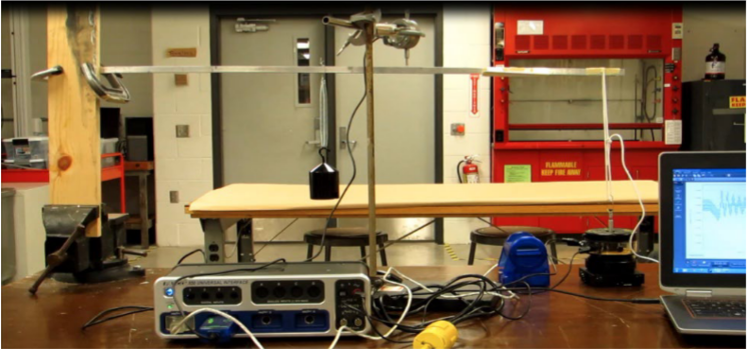
\includegraphics[width=6in]{images/Lab_Apparatus}
\caption{Lab apparatus completely set up, including the spring, weight, and displacement sensor. Image from the \textit{Lab 1 Practice Experiment and Data Analysis} manual \cite{lab_procedures}. Copyright 2023 by Thomas Chiou.}
\label{fig:lab_apparatus}
\end{figure}

As shown in Figure \ref{fig:lab_apparatus}, the left side of the beam is fixed to the board and the right side is attached to the wave driver with string. The rectangular, gray box in the foreground is the PASCO 850 Universal Interface, and the blue device in the midground is the motion sensor. The motion sensor must be positioned directly underneath the piece of white foam taped to the bottom of the beam with at least \qty{15}{cm} between the sensor and the foam.

\section{Procedures} \label{procedures}
\subsection{Setup} \label{procedures-setup}
Assemble the apparatus as described in Section \ref{apparatus}. Ensure that the styrofoam reflector plate is at least \qty{15}{cm} away from the motion sensor before running any tests. Launch the PASCO Capstone software, and turn on the PASCO 850 Universal Interface. Check that both the ``needle'' displacement sensor and motion sensors are recognized by the software. Once the sensors are recognized, configure the software to display two graphs ``by selecting the corresponding icon from the on-screen template'' \cite{lab_procedures}. Next, click on each axis to label the graphs, and set the y-label of the displacement sensor graph to ``displacement'' and ``position'' for the motion sensor graph. For both graphs, the x-label will be ``time''. Refer to Figure \ref{fig:pasco_main_page} to see how the graph layout should look.

\begin{figure}[ht]
\centering
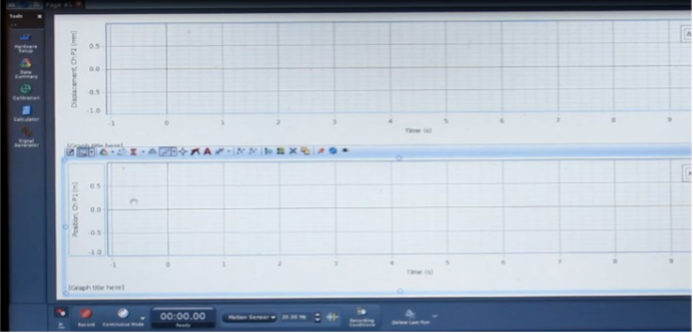
\includegraphics[width=5in]{images/PASCO_Main_Page}
\caption{The graph screen of the PASCO Capstone software fully configured for this lab. Image from the \textit{Lab 1 Practice Experiment and Data Analysis} manual \cite{lab_procedures}. Copyright 2023 by Thomas Chiou.}
\label{fig:pasco_main_page}
\end{figure}

Set up the wave driver by clicking the ``Signal Generator'' icon on the left-side of the screen.  Set the waveform to ``Sine'', sweep type to ``Off'', frequency to \qty{10}{Hz}, amplitude to \qty{10}{V}, and select ``Auto'' at the bottom of the window. For reference, compare your ``Signal Generator'' window to Figure \ref{fig:wave_driver_setup}.

\begin{figure}[ht]
\centering
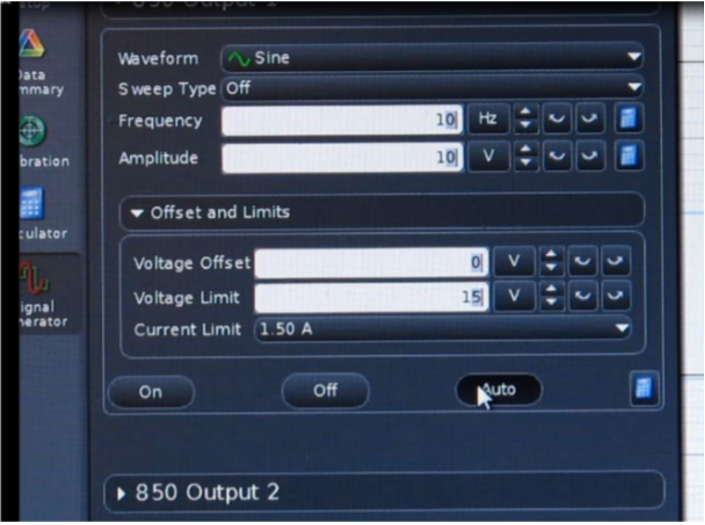
\includegraphics[width=4in]{images/Wave_Driver_Setup}
\caption{The wave driver or ``Signal Generator'' configuration window. Image from the \textit{Lab 1 Practice Experiment and Data Analysis} manual \cite{lab_procedures}. Copyright 2023 by Thomas Chiou.}
\label{fig:wave_driver_setup}
\end{figure}

Next, at the bottom of the screen select ``Recording Condition'', then select ``Stop Condition''. Set ``Condition Type'' to ``Time Based'', and set the time to \qty{15}{s}. The ``Recording Condition'' window will look similar to Figure \ref{fig:stop_conditions}. 

\begin{figure}[ht]
\centering
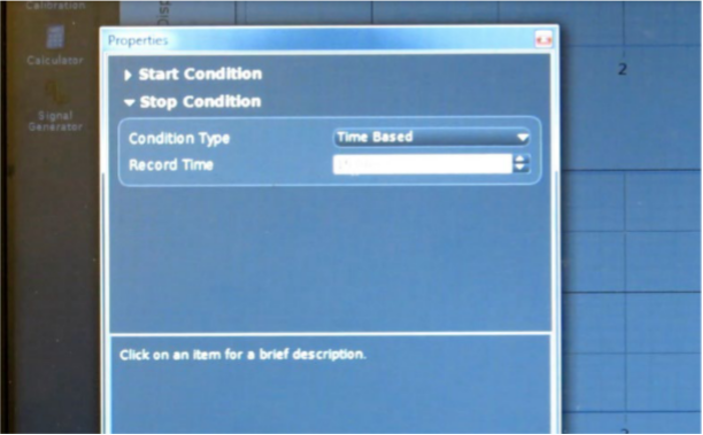
\includegraphics[width=4in]{images/Stop_Conditions}
\caption{The ``Stop Conditions'' configuration window. Image from the \textit{Lab 1 Practice Experiment and Data Analysis} manual \cite{lab_procedures}. Copyright 2023 by Thomas Chiou.}
\label{fig:stop_conditions}
\end{figure}

At the bottom of the screen, select ``Motion Sensor'', and set the sampling frequency to \qty{100}{Hz}. The sensor can be zeroed by selecting the icon to the right of the sampling frequency field. Use the same process to set up the displacement sensor, except set the sampling frequency to \qty{5}{Hz}. To zero the displacement sensor, click the physical O/I button on the sensor. The sensors should be zeroed before each round of testing.

Finally, navigate through the following menus: ``Data Summary'' icon on the left column of the screen $\rightarrow$ Motion Sensor $\rightarrow$ Position (m) $\rightarrow$ select the gear symbol $\rightarrow$ Numerical Format $\rightarrow$ change Number Style to Significant Figures $\rightarrow$ set the Number of Significant Figures to \num{5}. Follow the exact same process for the displacement sensor.

\subsection{Test 1} \label{procedures-test_1}
For Test 1, we will only utilize the wave driver. Take the hanging weight off the beam before starting and remain clear of the apparatus during operation. Ensure the displacement sensor is making good contact with the beam and approximately halfway depressed. Check the motion sensor is directly under the styrofoam reflector plate with at least \qty{15}{cm} of buffer. The string that attaches the beam to the axle socket of the wave driver should be taut. Lastly, double-check that the connector tip of the wave driver ``is firmly seated inside the axle socket'' \cite{lab_procedures}. Zero both sensors before running the test, then, in the PASCO Capstone software, click ``Record'' to run the test. Let the test run for the entire \qty{15}{s} duration. 

\subsection{Test 2} \label{procedures-test_2}
Before beginning Test 2, remove the displacement sensor from the beam and add the hanging weight to the spring. Begin the test as described in Section \ref{procedures-test_1}. As the test begins, a group member will pull the weight down and release it, allowing the spring-weight system to oscillate for the duration of the test. Be careful not to pull the weight down too hard.

\subsection{Test 3} \label{procedures-test_3}
For Test 3, leave the apparatus as it was configured for Test 2 in Section \ref{procedures-test_2}. Start the test as described in Section \ref{procedures-test_1}. After beginning the test, in addition to pulling down and releasing the hanging weight, a group member will randomly tap the free end of the cantilevered beam up or down every \numrange{2}{3} seconds for the duration of the test.

\subsection{Cleanup} \label{procedures-cleanup}
Using the ``File'' menu in the PASCO Capstone software, save the experiment data to a \texttt{.txt} or \texttt{.csv} file. Transfer the data to a flash drive for post-processing and analysis.

\section{Data} \label{data}
\subsection{Test 1} \label{data-test_1}


\subsection{Test 2} \label{data-test_2}


\subsection{Test 3} \label{data-test_3}


\chapter{Conclusion} \label{conclusion-chapter}
\section{Analysis} \label{analysis}


\section{Conclusion} \label{conclusion-section}


\printbibliography[heading=subbibintoc]

\appendix
\chapter{Graphs} \label{graphs}


\chapter{Code} \label{code}
\end{document}
